%% =========================================================================
%% Section 3: Data and Empirical Methodology
%% =========================================================================

\section{Data and Empirical Methodology}

\subsection{Data Source and Survey Population}
The empirical analysis is based on microdata from Wave 1 of the \textbf{Longitudinal Ageing Study in India (LASI)}, fielded between April 2017 and December 2018. LASI is a nationally representative, biennial longitudinal panel study designed to investigate the health, economic, and social consequences of population ageing in India. The study was jointly planned and executed by the International Institute for Population Sciences (IIPS), Mumbai, Harvard T.H. Chan School of Public Health, and the University of Southern California (USC).

LASI surveyed 73,396 individuals aged 45 and older and their spouses across all 36 States and Union Territories of India. To maintain a strict life-course gerontological focus, our target analytical population was restricted to adults aged 45 years and older ($N = 66{,}606$), systematically excluding 6,790 younger cohabiting spouses aged $<45$. Figure~\ref{fig:age_dist} illustrates the survey-weighted age distribution of this target population. Approximately 49.8\% of respondents are in mid-life (45--59 years), 38.8\% are in young-old adulthood (60--74 years), and 11.4\% are in the oldest-old stage (75 years and older).

\begin{figure}[!htbp]
    \centering
    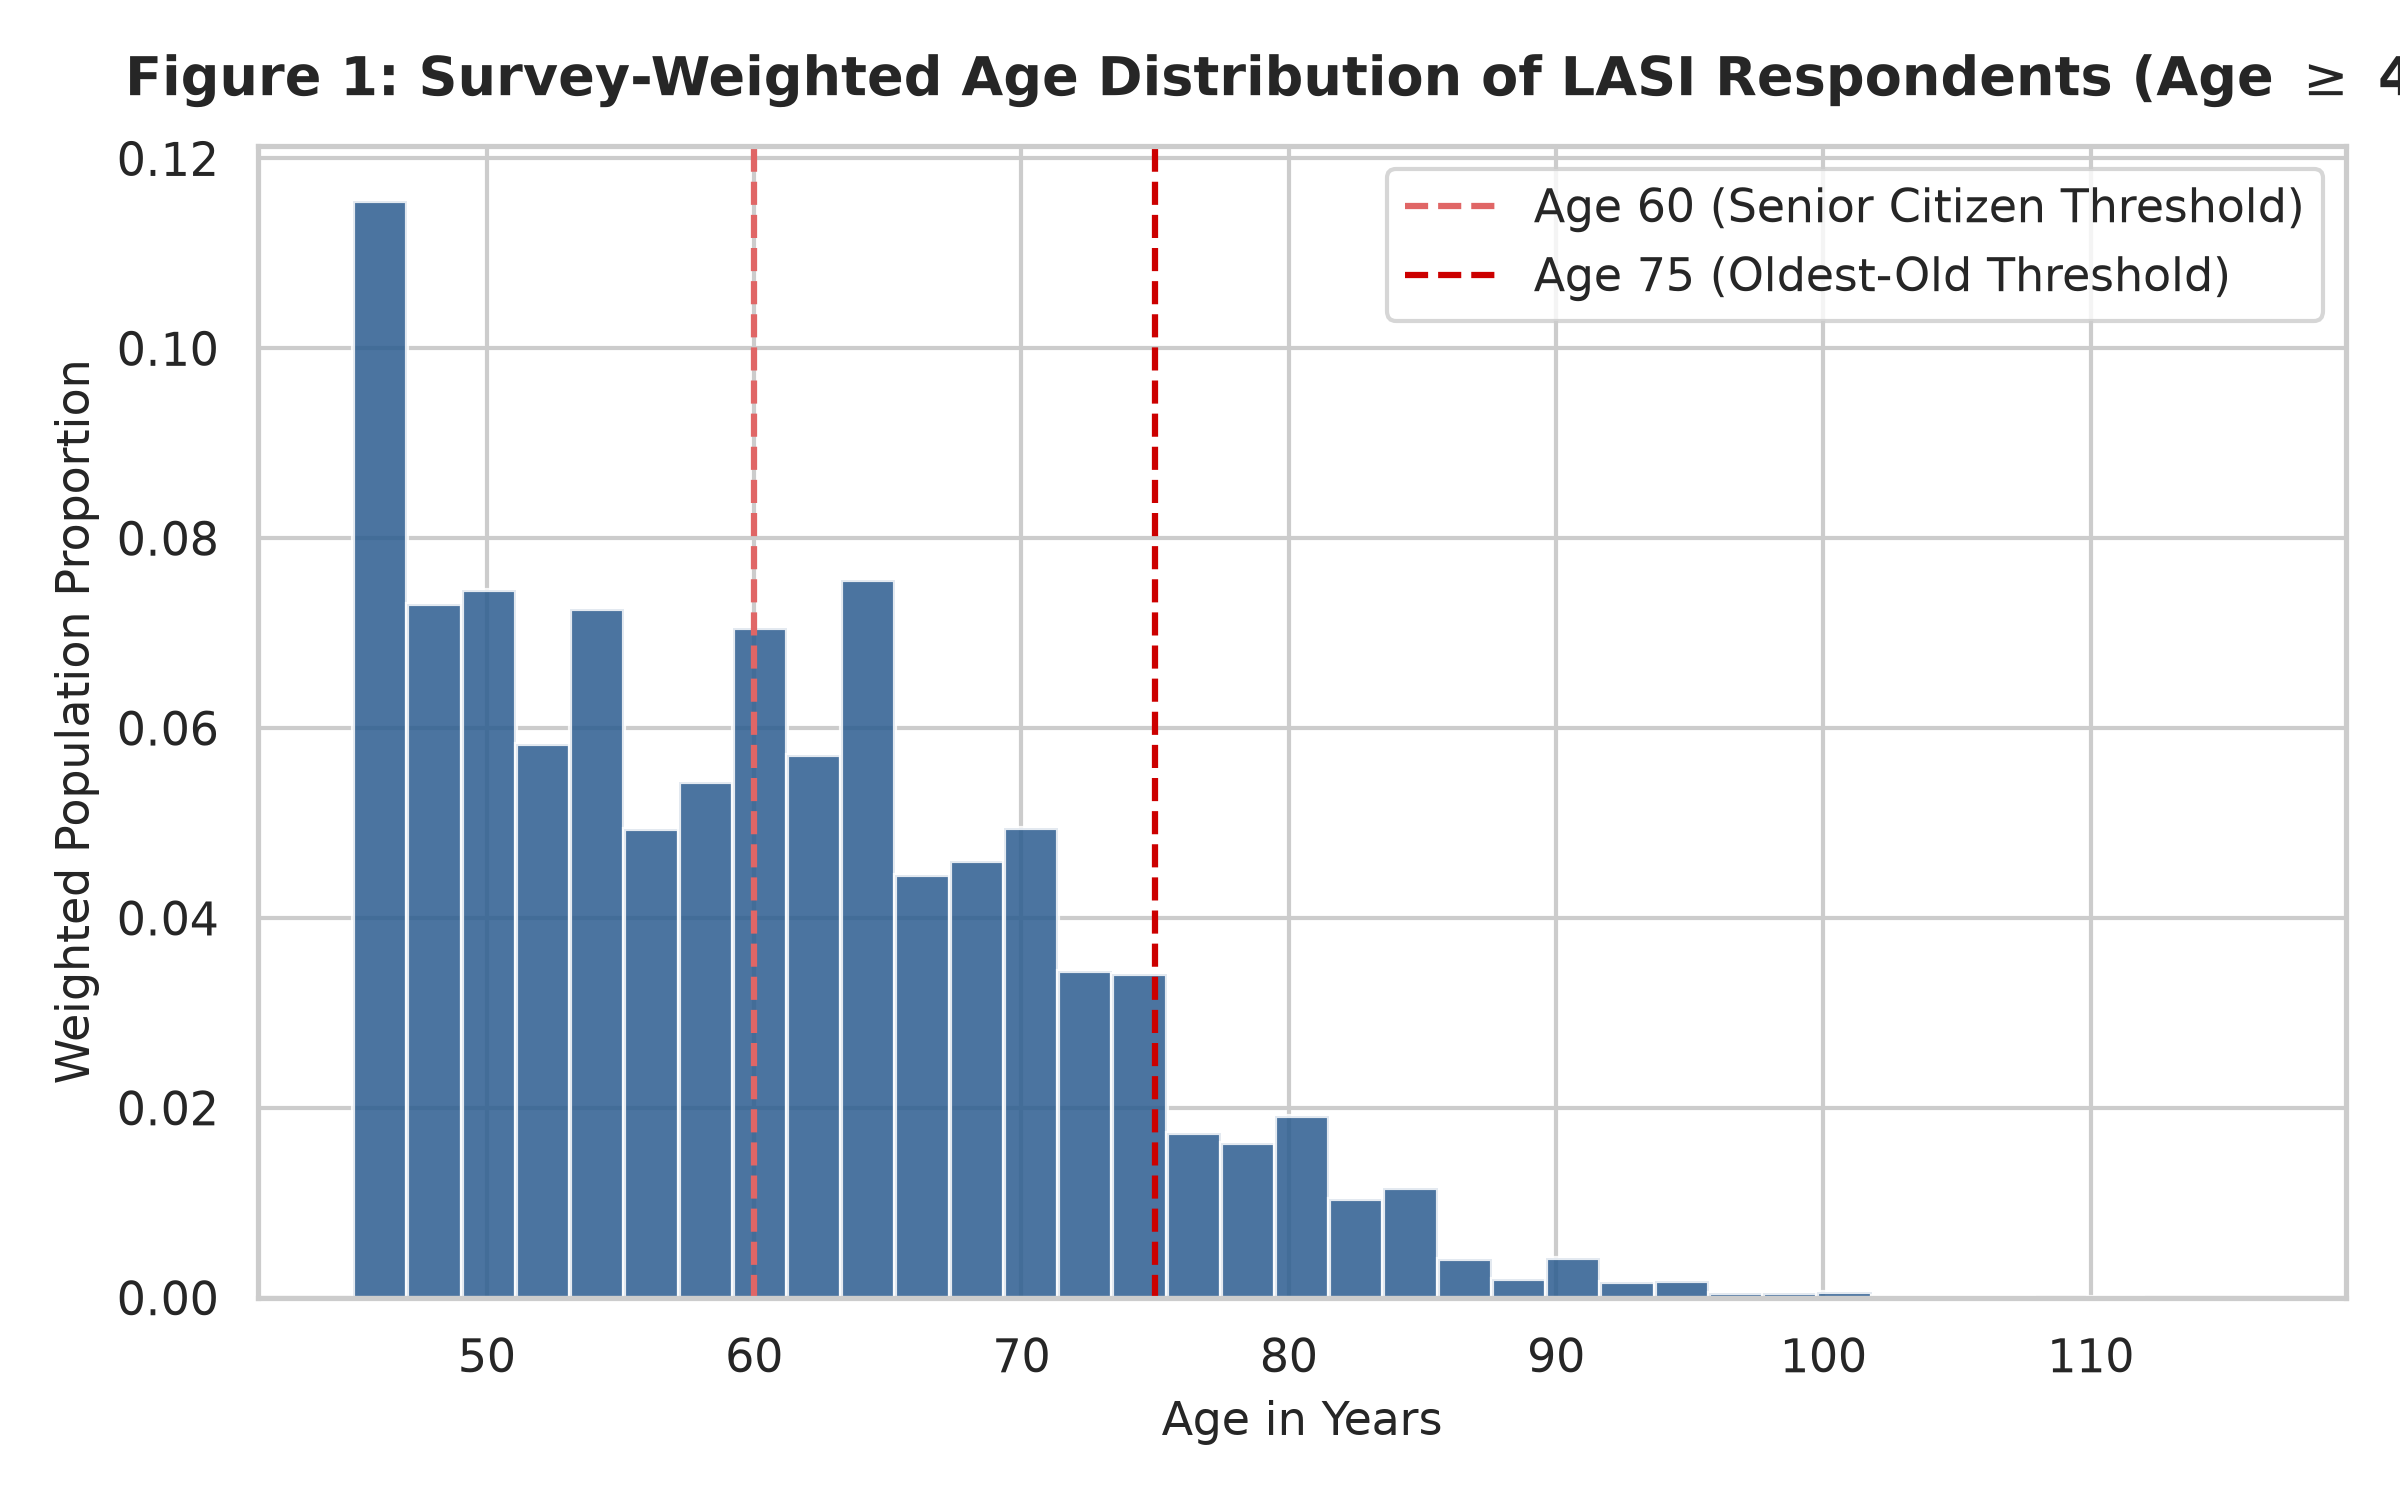
\includegraphics[width=0.82\textwidth]{figures/figure1_age_distribution.png}
    \caption{\textbf{Survey-Weighted Age Distribution of the Analytic Population ($\mathbf{N=66{,}606}$).} Shows the population distribution across five-year age intervals from age 45 to 90+, highlighting key demographic milestones.}
    \label{fig:age_dist}
\end{figure}

\subsection{Sampling Design and Survey Weighting}
LASI adopted a multi-stage stratified area probability cluster sampling design:
\begin{enumerate}[label=\alph*.]
    \item \textbf{Stratification (72 Strata):} Each of India's 36 States and Union Territories was stratified into rural and urban sectors, producing 72 independent geographic strata.
    \item \textbf{Clustering (2,428 Sampling Units):} In rural areas, sub-districts (tehsils) were selected as Primary Sampling Units (PSUs), and villages were sampled as Secondary Sampling Units (SSUIDs). In urban areas, wards were selected as PSUs, and Census Enumeration Blocks (CEBs) were selected as SSUIDs.
    \item \textbf{Survey Weights:} Individual-level post-stratification sampling weights (\texttt{indiaindividualweight}) were normalized and applied to all tabulations and statistical models to account for differential selection probabilities, non-response, and state population adjustments.
\end{enumerate}

\subsection{Operationalization of Early-Life Exposures}
Early-life circumstances experienced up to age 16 were ascertained through retrospective self-report modules in the individual questionnaire:

\begin{enumerate}
    \item \textbf{Childhood Socioeconomic Status (SES, \texttt{ht235}):} Respondents rated their family's financial situation while growing up before age 16:
    \begin{itemize}
        \item \textit{Pretty well-off financially} (Reference group: weighted 7.8\%, unweighted $N = 4,848$)
        \item \textit{About average} (Weighted 49.3\%, unweighted $N = 35,438$)
        \item \textit{Poor} (Disadvantaged group: weighted 42.2\%, unweighted $N = 25,605$)
        \item \textit{It varied} (Exploratory category: weighted 0.8\%, unweighted $N = 394$)
    \end{itemize}
    
    \item \textbf{Childhood General Health (\texttt{ht231}):} Evaluated via the question: ``Would you say that your health from birth up to age 16 was excellent, very good, good, fair, or poor?'' Following standard epidemiological practice, responses were categorized into:
    \begin{itemize}
        \item \textit{Good health} (Reference: Very good + Good; weighted 87.5\%, $N = 58,272$)
        \item \textit{Poor/Fair health} (Exposed: Fair + Poor + Very poor; weighted 12.5\%, $N = 7,369$)
        \item \textit{Sensitivity dichotomy:} In sensitivity checks matching certain published studies, we also tested a narrower collapse (Poor/Very poor [1.6\%] vs. Excellent/Very good/Good/Fair [98.4\%]).
    \end{itemize}

    \item \textbf{Childhood Bedridden Illness (\texttt{ht233}):} A binary indicator asking whether the respondent was ever confined to bed for one month or longer due to a severe health condition or accident before age 16 (Yes: weighted 5.8\%, $N = 3,370$; No: weighted 94.2\%, $N = 62,881$).

    \item \textbf{Cumulative Childhood Adversity Index:} An additive integer score ranging from 0 to 3, summing one point for poor childhood SES, one point for poor/fair childhood health, and one point for bedridden illness. In the target population, 48.2\% experienced 0 adversities, 44.1\% experienced 1 adversity, 6.9\% experienced 2 adversities, and 0.9\% experienced all 3 adversities (Figure~\ref{fig:child_prev}).
\end{enumerate}

\begin{figure}[!htbp]
    \centering
    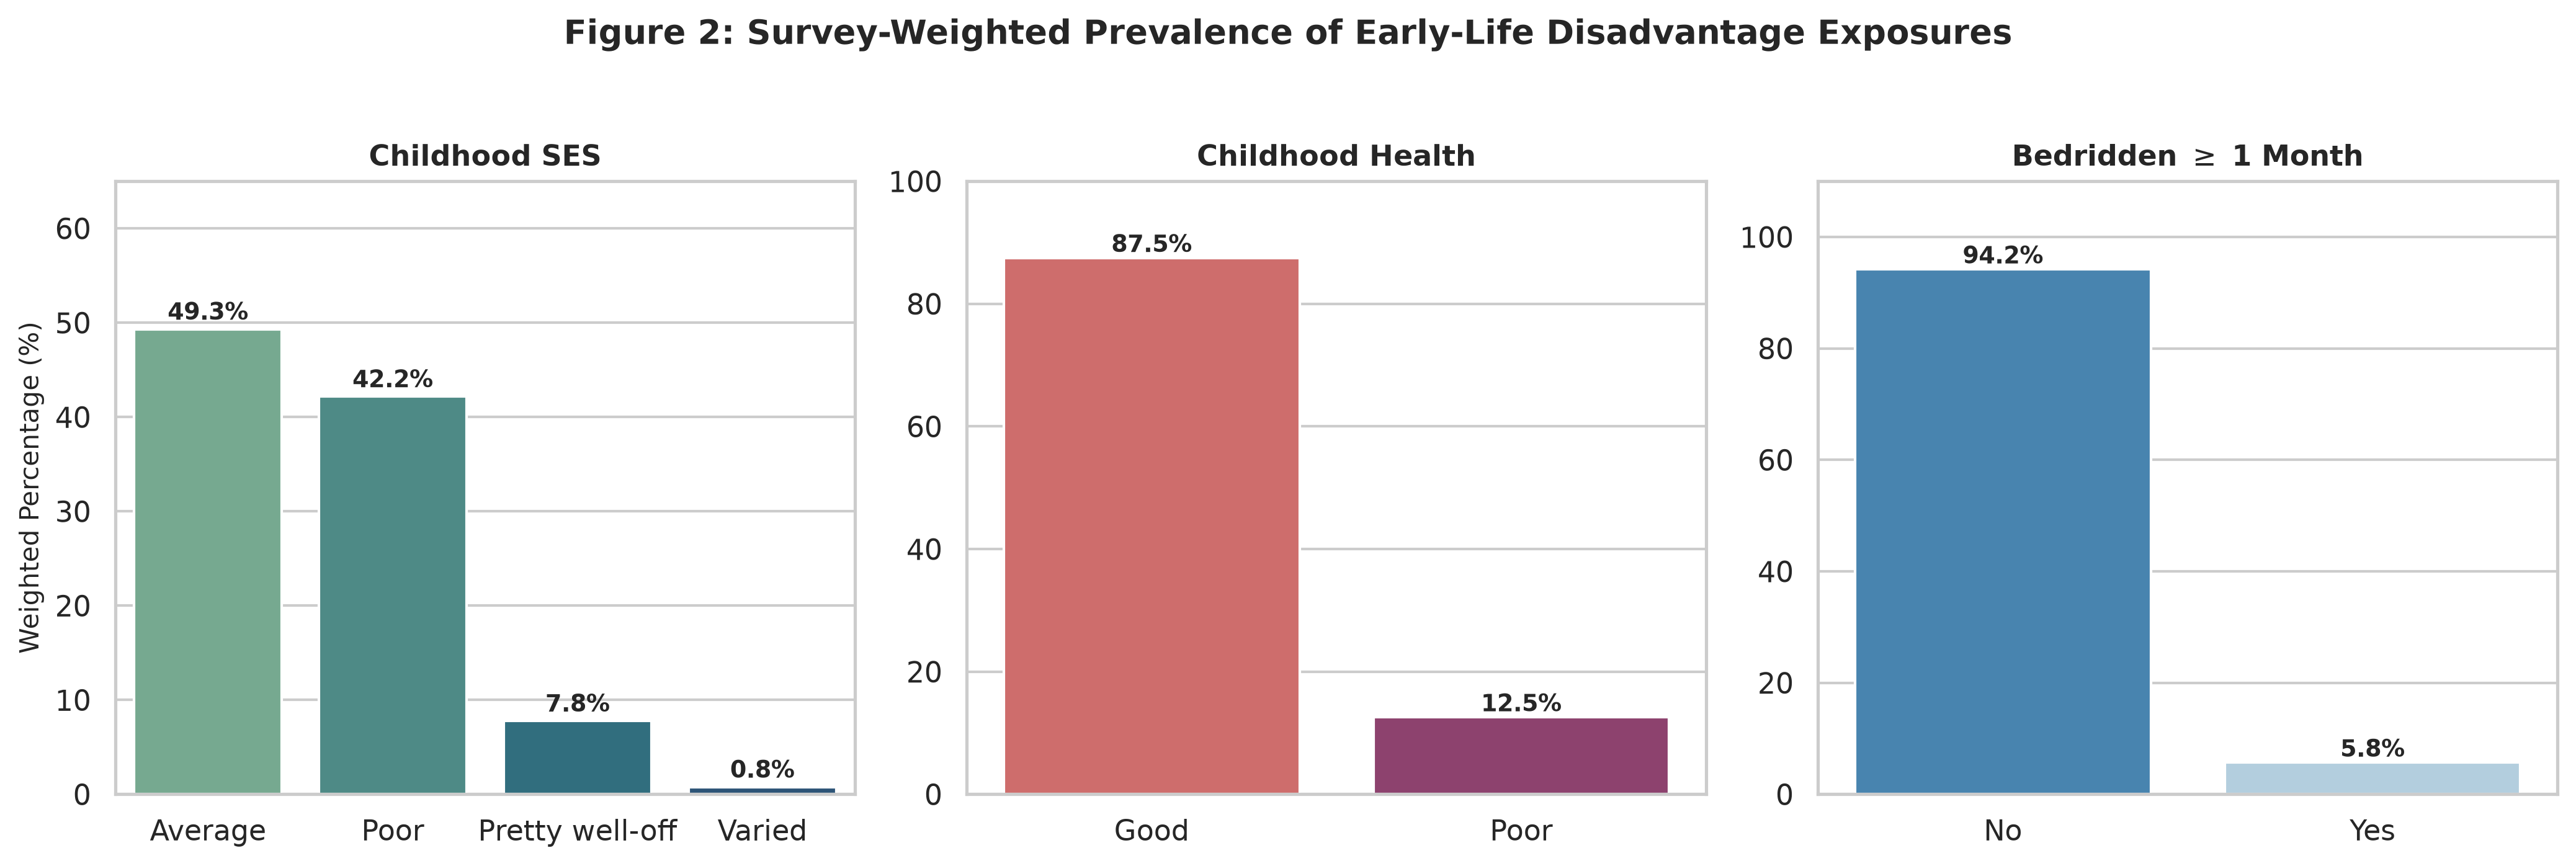
\includegraphics[width=0.82\textwidth]{figures/figure2_childhood_disadvantage_prevalence.png}
    \caption{\textbf{Survey-Weighted Prevalence of Early-Life Disadvantage Exposures ($\mathbf{N=66{,}606}$).} Shows the national proportion of older Indian adults reporting poor childhood SES (42.2\%), poor/fair childhood health (12.5\%), and prolonged bedridden illness (5.8\%).}
    \label{fig:child_prev}
\end{figure}

\subsection{Operationalization of Health Outcomes}

\subsubsection{Depressive Symptoms (10-Item CES-D)}
Late-life depressive symptoms were assessed using the 10-item version of the Center for Epidemiologic Studies Depression Scale (\texttt{fs701}--\texttt{fs710}). Respondents were asked about symptom frequency over the past week across seven negative affect items (depressed mood, low energy, restless sleep, loneliness, sadness, difficulty concentrating, feeling everything was an effort) and three positive affect items (feeling happy, hopeful, satisfied; reverse-coded). 

Responses were scored binary (0 = rarely/never; 1 = sometimes/often). For participants completing at least 8 of the 10 items, total scores were summed and proportionally scaled to a 0--10 continuum. Clinically significant depressive symptoms were defined using the established, internationally validated cutoff of $\text{CES-D} \ge 4.0$, yielding an unadjusted national weighted prevalence of \textbf{28.2\%} ($N = 64,825$ valid respondents).

\subsubsection{Cognitive Performance and Low Memory-Orientation Performance}
In LASI Wave 1, cognitive function was evaluated through an extensive neuropsychological battery covering episodic memory, orientation, arithmetic computation, executive functioning, and object naming. Non-proxy respondents ($N = 65,901$) were eligible for direct cognitive testing.

\paragraph{Addressing Item-Skip Bias in Cognitive Assessment:}
In the broader 43-point multi-domain cognitive battery, items involving mental arithmetic (serial 7s, backward counting) and graphic manipulation (overlapping pentagons, paper folding) were systematically skipped by interviewers for respondents without formal schooling to avoid respondent distress. If skipped questions are treated as zero points (failures), the resulting composite functions largely as an artificial indicator of formal schooling (Figure~\ref{fig:edu_grad} and Table~\ref{tab:edu_gradient}). 

\begin{figure}[!htbp]
    \centering
    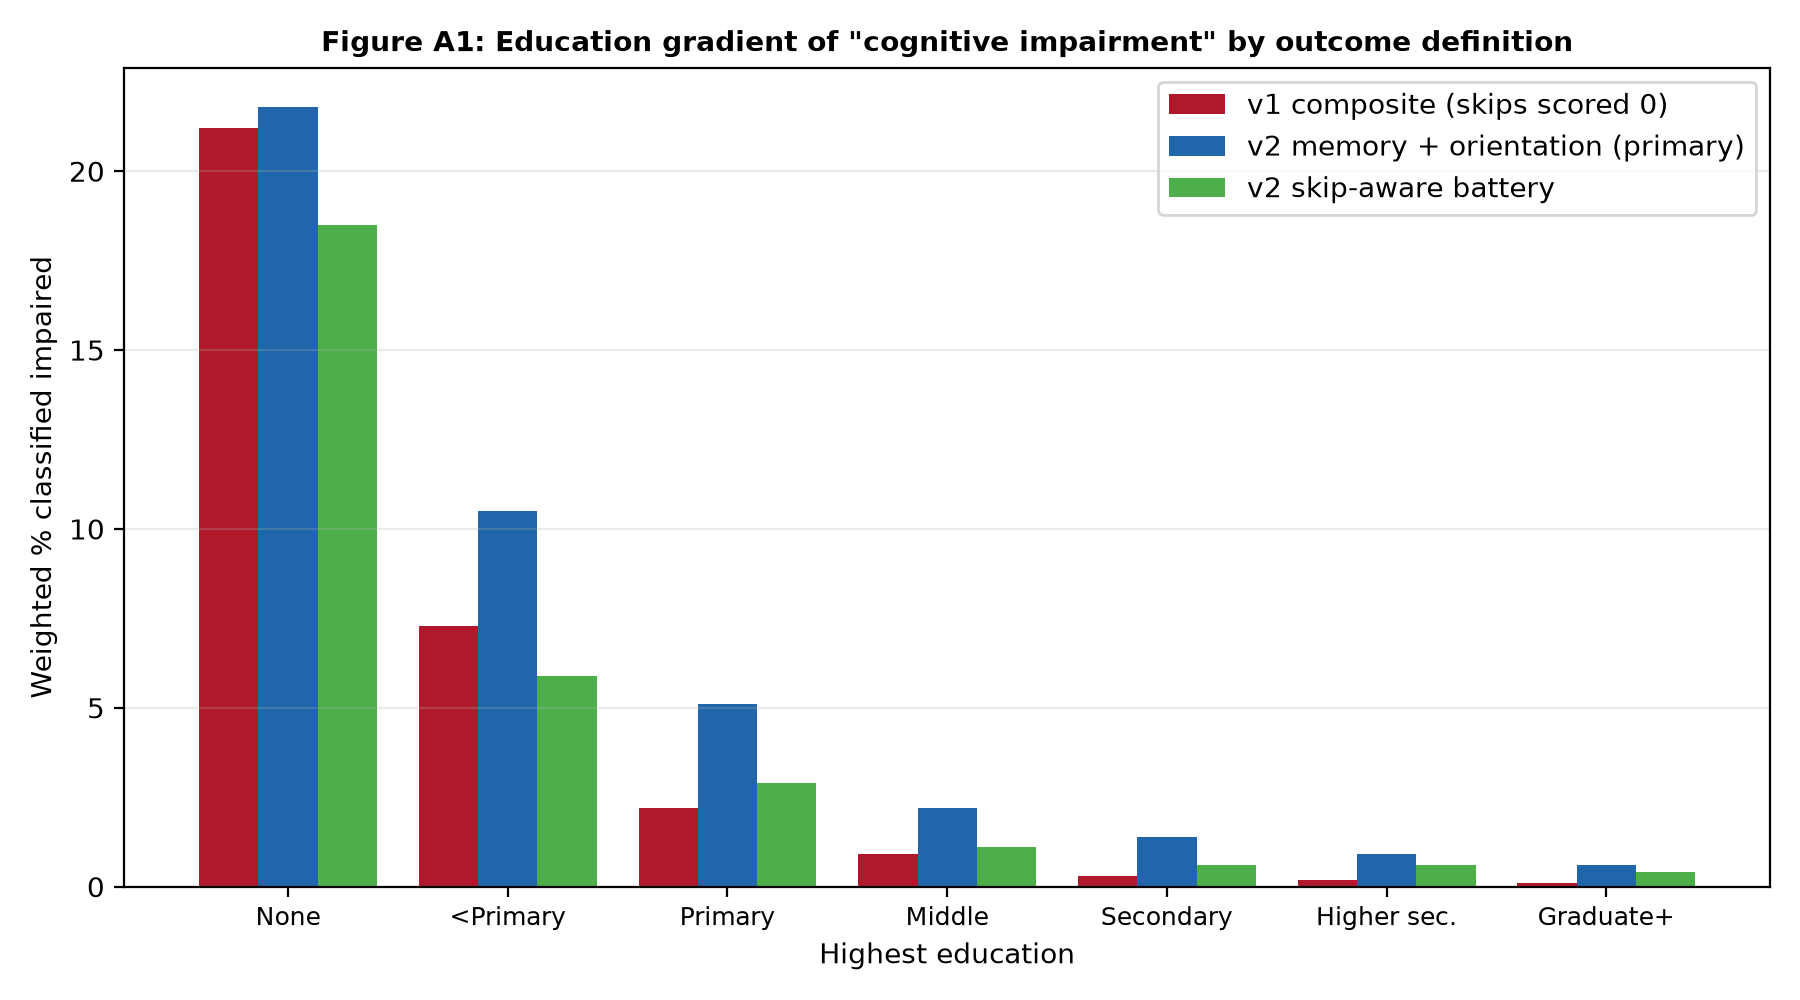
\includegraphics[width=0.82\textwidth]{figures/figureA1_education_gradient.png}
    \caption{\textbf{Impact of Cognitive Battery Construction across Educational Strata.} The unadjusted multi-domain composite (scoring skipped arithmetic tasks as 0) showed an extreme artificial cliff for unschooled adults. The memory-and-orientation composite establishes an education-fair measurement basis.}
    \label{fig:edu_grad}
\end{figure}

\begin{table}[!htbp]
\centering
\small
\caption{\textbf{Cognitive Impairment Prevalence (\%) across Educational Strata under Alternative Battery Formulations.}}
\label{tab:edu_gradient}
\resizebox{0.92\textwidth}{!}{%
\begin{tabular}{lcccc}
\toprule
\textbf{Educational Attainment} & \textbf{Analytic N} & \textbf{Literacy-Confounded (\%)} & \textbf{Skip-Aware Full Battery (\%)} & \textbf{Memory + Orientation (\%)} \\
\midrule
No formal education             & 26,760 & 21.2\% & 18.5\% & 21.8\% \\
Less than primary               &  6,829 &  7.3\% &  5.9\% & 10.5\% \\
Primary completed               &  8,147 &  2.2\% &  2.9\% &  5.1\% \\
Middle completed                &  5,993 &  0.9\% &  1.1\% &  2.2\% \\
Secondary completed             &  5,681 &  0.3\% &  0.6\% &  1.4\% \\
Higher secondary / Diploma      &  3,056 &  0.2\% &  0.6\% &  0.9\% \\
Graduate and above              &  3,314 &  0.1\% &  0.4\% &  0.6\% \\
\bottomrule
\end{tabular}%
}
\end{table}

To eliminate this measurement artifact, the primary cognitive outcome was established as the \textbf{Memory and Orientation Composite (0--28 points)}:
\begin{itemize}
    \item \textbf{Episodic Memory (0--20 points):} Immediate recall of a 10-word list (0--10 points) plus delayed recall of the same list after a short cognitive delay (0--10 points). Words were common, concrete nouns administered verbally in the respondent's native language.
    \item \textbf{Temporal and Spatial Orientation (0--8 points):} Awareness of current date, month, year, day of the week, place of interview, village/town, district, and state. Strict complete-case scoring required answers to all 8 questions.
\end{itemize}

Binary \textbf{Low Memory-Orientation Performance} was defined as scoring at or below the survey-weighted 10th percentile cutoff in the target population ($\le 11.0$ points), yielding a national weighted prevalence of \textbf{12.8\%} ($N = 59,781$ valid complete tests). 

\paragraph{Handling Informative Missingness:}
As shown in Figure~\ref{fig:cog_miss}, missingness in direct cognitive assessments was not random; it reached 19.9\% among adults aged 75+ and 13.3\% among unschooled individuals. To ensure that complete-case analysis did not introduce selection bias, we implemented Inverse-Probability Weighting (IPW) as a sensitivity test, upweighting complete tests according to their predicted probability of observation.

\begin{figure}[!htbp]
    \centering
    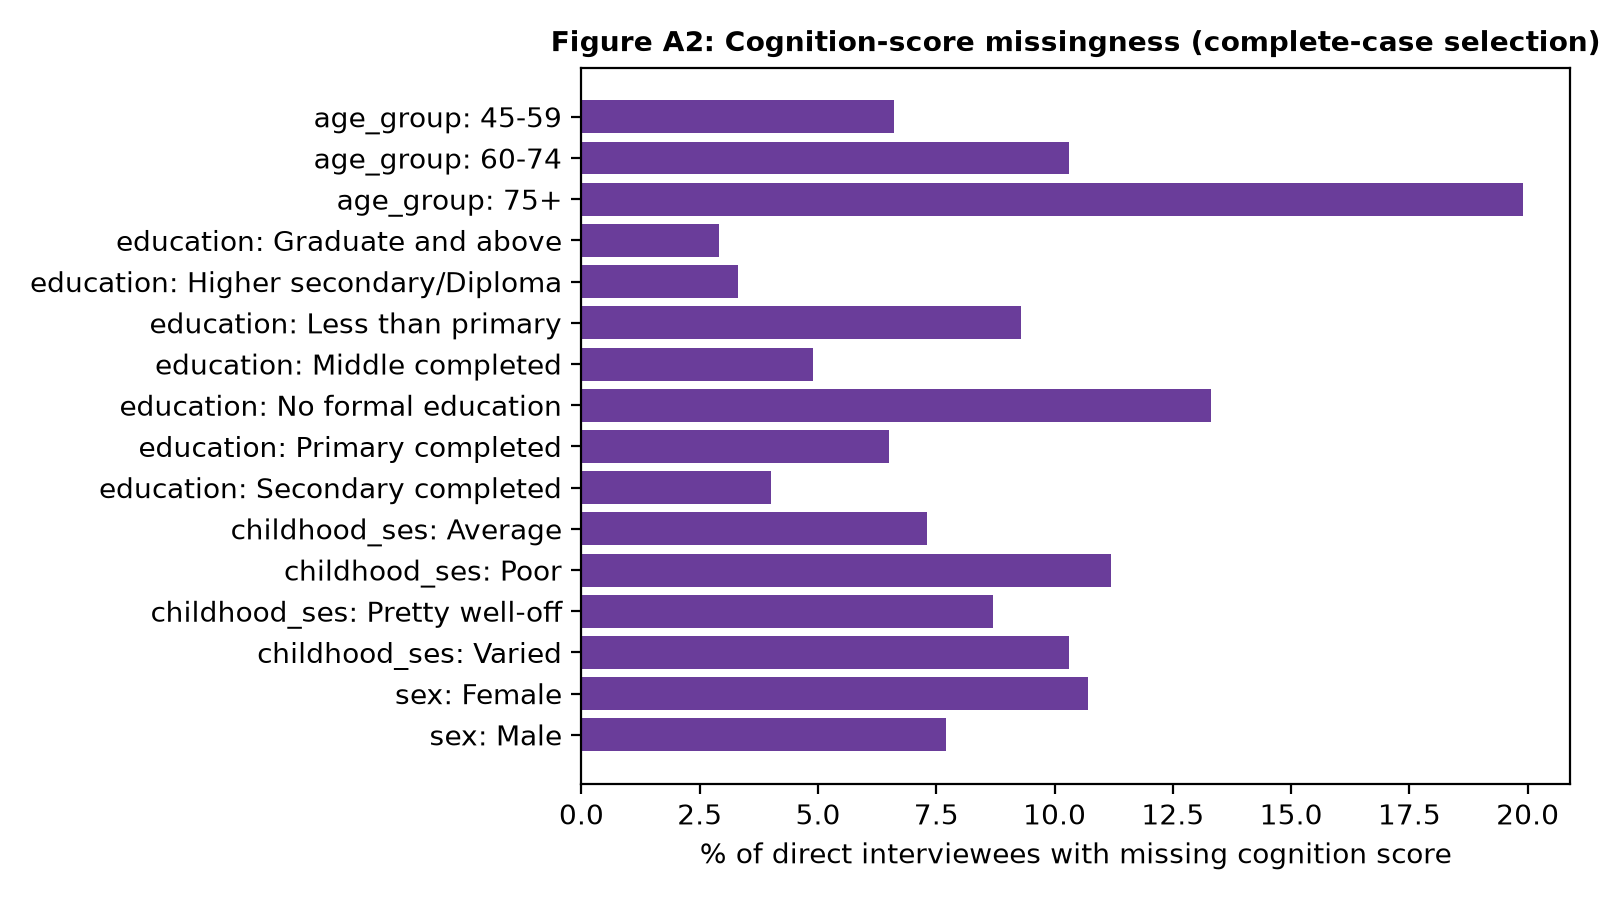
\includegraphics[width=0.82\textwidth]{figures/figureA2_cognition_missingness.png}
    \caption{\textbf{Proportion of Incomplete Cognitive Assessment Scores across Demographic Subgroups.} Missingness is concentrated among the oldest-old (75+) and illiterate elders, motivating our IPW robustness models.}
    \label{fig:cog_miss}
\end{figure}

\subsection{Model Hierarchy and Statistical Estimation}

\subsubsection{Modified Poisson Regression for Common Outcomes}
Because depressive symptoms (28.2\%) and cognitive impairment (12.8\%) are common binary outcomes, traditional logistic regression Odds Ratios would substantially overestimate the true relative risk. We utilized survey-weighted \textbf{Modified Poisson Regression} with a logarithmic link function and robust sandwich standard errors to estimate adjusted \textbf{Prevalence Ratios (PR)} and 95\% Confidence Intervals:
\begin{equation}
    \log \left( \mathbb{E}[Y_i \mid \mathbf{X}_i] \right) = \beta_0 + \sum_{k} \beta_k X_{ik}
\end{equation}
A Prevalence Ratio directly indicates relative risk: an APR of $1.20$ denotes a 20\% higher prevalence of the condition in the exposed group compared to the reference group.

\subsubsection{Stratified Cluster Sandwich Variance Estimation}
Standard errors were calculated using design-based Taylor series linearization accounting for the multi-stage cluster design across 72 strata and 2,428 Primary Sampling Units (clusters). The cluster-robust sandwich covariance matrix was calculated as:
\begin{equation}
    \mathbf{V} = \left( \mathbf{X}^T \mathbf{W} \mathbf{X} \right)^{-1} \mathbf{S} \left( \mathbf{X}^T \mathbf{W} \mathbf{X} \right)^{-1}
\end{equation}
where $\mathbf{S}$ represents the between-cluster sum of score residuals centered within each stratum $h$:
\begin{equation}
    \mathbf{S} = \sum_{h=1}^{H} \frac{n_h}{n_h - 1} \sum_{c=1}^{n_h} \left( \mathbf{u}_{hc} - \bar{\mathbf{u}}_h \right) \left( \mathbf{u}_{hc} - \bar{\mathbf{u}}_h \right)^T
\end{equation}
Hypothesis tests were evaluated against the Student's $t$-distribution with survey degrees of freedom $df = \sum n_h - H = 2,428 - 72 = 2,356$.

\subsubsection{Common Complete-Case Sample and Model Sequence}
To ensure that changes in estimated coefficients across models reflect true confounding or attenuation rather than sample attrition, all nested models were estimated on invariant common complete-case samples (Table~\ref{tab:common_samples}).

\begin{table}[!htbp]
\centering
\small
\caption{\textbf{Analytic Invariance: Common Complete-Case Sample Sizes across Sequential Models.}}
\label{tab:common_samples}
\begin{tabular}{lcccc}
\toprule
\textbf{Outcome Analysis Domain} & \textbf{Analytic Sample N} & \textbf{PSUs (Clusters)} & \textbf{Sampling Strata} & \textbf{Survey Degrees of Freedom} \\
\midrule
Cognitive Impairment (Memory + Orientation) & 57,245 & 2,428 & 72 & 2,356 \\
Depressive Symptoms (CES-D $\ge 4$)          & 62,047 & 2,428 & 72 & 2,356 \\
\bottomrule
\end{tabular}
\end{table}

The sequential model hierarchy was defined as follows:
\begin{itemize}
    \item \textbf{Model 0 (Unadjusted):} Outcome $\sim$ Childhood Exposure.
    \item \textbf{Model A (Demographic + Regional Fixed Effects):} Model 0 + Continuous Age + Sex (Male vs. Female) + Sector (Rural vs. Urban) + Social Group / Caste (General/None, SC, ST, OBC, Other) + Marital Status (Married vs. Non-Married) + \textbf{36 State Fixed Effects}.
    \item \textbf{Model B (Adult SES -- Primary Model):} Model A + Educational Attainment (7 categories: No formal education, Less than primary, Primary, Middle, Secondary, Higher secondary/Diploma, Graduate and above) + Monthly Per Capita Consumption Expenditure (MPCE) Quintiles (Quintile 1 poorest to Quintile 5 richest).
    \item \textbf{Model C (Adult Health Pathway -- Exploratory):} Model B + Chronic Physical Morbidity Count (hypertension, diabetes, chronic lung disease, heart disease, stroke: 0 to 5) + Current Self-Rated Health (Excellent, Very good, Good, Fair, Poor).
\end{itemize}
